
Every effort has been made to ensure that building
the \efloat\ system is straightforward.
The default build supports execution of the test suite
with the selected \efloatclass\ type.
Simple operations or other spot--tests can be carried out by deactivating
the subroutine
{\courier{::test{\ttfamily{\underline\ }}real{\ttfamily{\underline\ }}imag}}
and activating the subroutine
{\courier{test::spot::test{\ttfamily{\underline\ }}spot}}
in the {\courier main} program which is implemented in the
file {\courier {test/test.cpp}}.
Designers of advanced applications can remove the test suite entirely
and create a custom build.

\subsection{Compiler Systems}

\begin{table}[ht]\noindent
\begin{center}
\renewcommand{\arraystretch}{1.15}
\begin{tabular}{c|c|c|c}

Compiler
            & Compatible
            & Final Test
            & Build System \\

\hline

Microsoft{\footnotesize {\textregistered}}~Visual~C++{\footnotesize {\textregistered}}~x86
            & \multirow{2}{*}{$\ge 9$ with SP1}
            & \multirow{2}{*}{9 with SP1}
            & \multirow{2}{*}{Microsoft{\footnotesize {\textregistered}} NMAKE} \\

Microsoft{\footnotesize {\textregistered}}~Visual~C++{\footnotesize {\textregistered}}~x64
            & & & \\

\hline

GNU$\,\,$GCC~i686--pc--cygwin
            & \multirow{2}{*}{$\ge 4$.$2$.$2$}
            & \multirow{2}{*}{$4$.$4$.$2$}
            & \multirow{2}{*}{GNUmake $3$.$81$} \\

GNU$\,\,$GCC~x$86${\ttfamily\underline\ }$64$--linux--gnu
            & & & \\

\hline

Intel{\footnotesize {\textregistered}}~ICC~x86
            & \multirow{2}{*}{$\ge 11$.$1$.$046$}
            & \multirow{2}{*}{$11$.$1$.$051$}
            & \multirow{2}{*}{Microsoft{\footnotesize {\textregistered}} NMAKE} \\

Intel{\footnotesize {\textregistered}}~ICC~x64
            & & & \\

\hline

\end{tabular}
\vspace{2.0mm}
\caption{The compilers and build systems supported by \efloat\ are shown.}
\label{table:compilers}
\end{center}
\end{table}



Several compiler systems have been used at their highest warning settings
in order to achieve very high levels of language standards adherence,
portability and reliability.
The compilers and build systems in Table~\ref{table:compilers}
have been used to develop, build and test \efloat.
Tools from Microsoft{\footnotesize {\textregistered}}, Intel{\footnotesize {\textregistered}}
and GNU are supported
(see~\cite{microsoft:vs2008,microsoft:nmake,icc:website,gcc:website,gnumake:website}).
The tools in the ``Compatible'' column have been used
to successfully build and execute the system.
Those in the ``Final Test'' column have been used not only to
successfully build and execute the system, but also to test and
verify \efloat\ using the entire test suite
for three different MP types, each tested at
$30$, $50$, $100$, $200$ and $300$ digits of precision.

\pagebreak

\subsection{Windows{\footnotesize {\textregistered}} Environment}

\begin{figure}[ht]
\centering
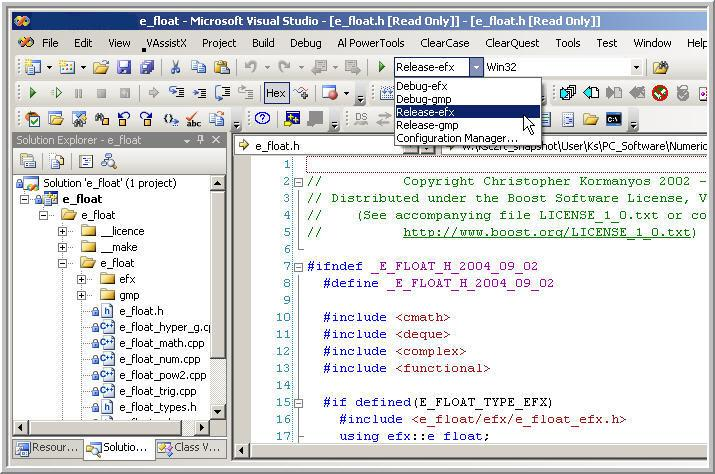
\includegraphics[width=16.0cm]{ef_man_Graphic_200_DevStudioConfig.jpg}
\vspace{0.4cm}
\caption{The \efloat\ configuration selection with Microsoft{\footnotesize {\textregistered}}
Visual Studio{\footnotesize {\textregistered}} 2008 Professional ($+$SP1) is shown. The
project configurations listed in Table \ref{table:systemconfigs} can be selected and built.}
\label{fig:devstudioconfig}
\end{figure}

\noindent \efloat\ can be built within a Windows{\footnotesize {\textregistered}} environment
using Microsoft{\footnotesize {\textregistered}} Visual Studio{\footnotesize {\textregistered}}
2008 Professional with Service Pack $1$ (SP$1$), as shown in Figure~\ref{fig:devstudioconfig}.

\subsubsection{Building the Configurations `efx', `gmp', `mpfr' and `f90' in Windows{\footnotesize {\textregistered}}}

\begin{itemize}
\item Open the solution workspace file
{\courier e\underline\ float/e\underline\ float.sln},
as shown in Figure \ref{fig:devstudioconfig}.
\item Select the appropriate project configuration such as
``release--mpfr'', as shown in Figure \ref{fig:devstudioconfig}
(see Table \ref{table:systemconfigs}).
\item Select 32--bit or 64--bit targets by selecting either ``Win32'' or ``x64'' using
the ``Solution Platforms'' manager.
\item Build the solution with the menu item {\courier Build}$\dots${\courier Build Solution},
or use the corresponding build button.
\item Rebuild the solution with the menu item {\courier Build}$\dots${\courier Rebuild Solution},
or use the corresponding rebuild button.
\item The configurations {\courier gmp} and {\courier mpfr} require GNU~MP and GNU~MP~$+$~MPFR,
respectively. Therefore, GNU MP and MPFR have been ported to
Microsoft{\footnotesize {\textregistered}} Visual Studio{\footnotesize {\textregistered}} 2008
and built for the Windows{\footnotesize {\textregistered}} environment,
based in part on the original porting work provided by
Gladman \cite{gladman:ports}. Separate builds are provided for the 32--bit
Intel{\footnotesize {\textregistered}}
IA32 architecture as well as the 64--bit
Intel{\footnotesize {\textregistered}} Core\ensuremath{^{\text{\courier TM}}}2
architecture (x64). The pre\-built libraries {\courier gmp}.{\courier lib} and {\courier mpfr}.{\courier lib}
for both IA32 as well as x64 have been copied to the respective directories
{\courier p4} and {\courier x64}, which  are subdirectories of the directory
{\courier e\underline\ float/gmp/4-2-4/vc9}. The link commands are already
present within the project file.
\item The configuration {\courier f90} requires the Fortran $90$ wrapper as well as the
corresponding Fortran run--time libraries to be linked with the project.
The Fortran $90$ wrapper {\courier libf90quad}.{\courier lib} has been prebuilt
for both IA32 as well as for x64 using the Intel{\footnotesize {\textregistered}}
Fortran compiler. In addition, the Fortran run--time libraries have been extracted from the
Intel{\footnotesize {\textregistered}} Fortran installation directories for both
IA32 as well as x64.
All of these libraries are stored in the respective directories
{\courier p4} and {\courier x64}, which  are subdirectories of
{\courier e\underline\ float/}{\courier f90/libf90quad/vc9}.
The necessary link commands are already present within the
Microsoft{\footnotesize {\textregistered}} Visual Studio{\footnotesize {\textregistered}}
project file.
\end{itemize}


\subsubsection{Building the Configuration `clr' in Windows{\footnotesize {\textregistered}}}

\begin{itemize}
\item Open the solution workspace file
{\courier e\underline\ float/e\underline\ float.sln},
\item Select the project configuration ``release--clr''.
\item Build the solution with the menu item {\courier Build}$\dots${\courier Build Solution},
or use the corresponding build button.
\item Rebuild the solution with the menu item {\courier Build}$\dots${\courier Rebuild Solution},
or use the corresponding rebuild button.
\item This build configuration produces a
Microsoft{\footnotesize {\textregistered}} Windows{\footnotesize {\textregistered}}~.NET
assembly which can be used with any .NET language in the
Microsoft{\footnotesize {\textregistered}}~CLR.
\end{itemize}

\subsubsection{Building the Configuration `pyd' in Windows{\footnotesize {\textregistered}}}

\begin{itemize}
\item Open the solution workspace file
{\courier e\underline\ float/e\underline\ float.sln},
\item Select the project configuration ``release--pyd''.
\item Build and rebuild the solution as described above.
\item This configuration is only available for the Win32 platform.
\end{itemize}

\subsubsection{Building the Configuration `cas' in Windows{\footnotesize {\textregistered}}}

\begin{itemize}
\item This configuration depends strongly on the selected computer algebra system.
\item An example in given for Mathematica{\footnotesize {\textregistered}}~7.1
for the Win32 platform.
\item Contact the author for detailed instructions when interfacing with
a computer algebra system.
\end{itemize}

\subsection{UNIX--like Environment}

\efloat\ can be built within a UNIX--like environment, such as native UNIX,
native Linux, mingw or cygwin. Building \efloat\ within a UNIX--like
environment requires GCC version $4$.$3$.$1$ or higher
and GNUmake version $3$.$81$ or higher.
In order to successfully build \efloat\ with GCC, it must be verified that
both the version of GCC as well as the version of GNU make are high enough.
These checks can be done by querying the version of GCC (or g$++$) and the
version of GNUmake as shown below.

\vspace{6.0pt}

\lstsetBash
\begin{lstlisting}
chris@desktop:~$ g++ --version
g++ (GCC) 4.3.3
Copyright (C) 2008 Free Software Foundation, Inc.
...
\end{lstlisting}

\vspace{6.0pt}

\lstsetBash
\begin{lstlisting}
chris@desktop:~$ make --version
GNU make 3.81
Copyright (C) 2006 Free Software Foundation, Inc.
...
\end{lstlisting}

\subsubsection{Building the Configurations `efx', `gmp' and `mpfr' in UNIX}

\begin{itemize}
\item For UNIX--like operating systems, \efloat\ can be built using either of the
three MP implementations, {\courier efx}, {\courier gmp} or {\courier mpfr}.
\item The makefile is designed to accept the selection of the {\courier MP} type as an
input parameter, using either {\courier MP$=$efx} or {\courier MP$=$gmp}.
If the {\courier MP} flag is not provided, the default behavior is to build
with {\courier MP$=$efx}.
\item After entering the make command ({\it i.e.} starting the build), the build of the
project should begin and run successfully to completion.
\item The {\courier gmp} build configuration of \efloat\ requires an installed version of GNU MP
because it links with {\courier libgmp.lib} from the GNU MP ({\it i.e.} uses the
link command line switch $-${\courier lgmp}).
\item The {\courier mpfr} build configuration of \efloat\ requires installed versions of GNU~MP
as well as GNU~MP~$+$~MPFR because it links with {\courier libgmp.lib} and {\courier libmpfr.lib} 
({\it i.e.} uses the link command line switches $-${\courier lgmp} $-${\courier lmpfr}).
\end{itemize}

\noindent A sample build command line using {\courier efx::e\underline\ float} is shown in
the command line sequence of the sample bash session below.

\vspace{6.0pt}

\lstsetBash
\begin{lstlisting}
chris@desktop:~$ cd e_float
chris@desktop:~$ make MP=efx
\end{lstlisting}

\noindent A sample build command line using {\courier gmp::e\underline\ float} is shown in
the command line sequence of the sample bash session below.

\vspace{6.0pt}

\lstsetBash
\begin{lstlisting}
chris@desktop:~$ cd e_float
chris@desktop:~$ make MP=gmp
\end{lstlisting}

\noindent The {\courier clean} option of the \efloat\ build is also supported.
Be sure to use the correct value of the build flag {\courier MP} for clean
operations because the clean only cleans intermediate build results of the
selected build configuration. A sample build command line for cleaning the
project with the configuration {\courier gmp} is shown in the bash command
line sequence below.

\vspace{6.0pt}

\lstsetBash
\begin{lstlisting}
chris@desktop:~$ cd e_float
chris@desktop:~$ make clean MP=gmp
\end{lstlisting}


\subsubsection{Building the Configuration `clr' in UNIX}

The {\courier clr} configuration is not currently supported in UNIX.

\subsubsection{Building the Configuration `pyd' in UNIX}

\begin{itemize}
\item Build, rebuild and clean the solution using {\courier{make}}
with the make option {\courier{MP=pyd}}. A dynamic library is built.
\item This build links with the boost python library and the python library
as shown in the makefile. Ensure that these libraries
are properly installed for this build.
\end{itemize}

\subsubsection{Building the Configuration `cas' in Windows{\footnotesize {\textregistered}}}

The {\courier cas} configuration is not currently supported in UNIX.
Specialized support must be developed for the desired computer algebra system.

